\documentclass{article}

  % packages
    % basic stuff for rendering math
    \usepackage[letterpaper, top=1in, bottom=1in, left=1in, right=1in]{geometry}
    \usepackage[utf8]{inputenc}
    \usepackage[english]{babel}
    \usepackage{amsmath} 
    \usepackage{amssymb}
    \usepackage{amsthm}

    % extra math symbols and utilities
    \usepackage{mathtools}        % for extra stuff like \coloneqq
    \usepackage{mathrsfs}         % for extra stuff like \mathsrc{}
    \usepackage{centernot}        % for the centernot arrow 
    \usepackage{bm}               % for better boldsymbol/mathbf 
    \usepackage{enumitem}         % better control over enumerate, itemize
    \usepackage{hyperref}         % for hypertext linking
    \usepackage{fancyvrb}          % for better verbatim environments
    \usepackage{newverbs}         % for texttt{}
    \usepackage{xcolor}           % for colored text 
    \usepackage{listings}         % to include code
    \usepackage{lstautogobble}    % helper package for code
    \usepackage{parcolumns}       % for side by side columns for two column code
    

    % page layout
    \usepackage{fancyhdr}         % for headers and footers 
    \usepackage{lastpage}         % to include last page number in footer 
    \usepackage{parskip}          % for no indentation and space between paragraphs    
    \usepackage[T1]{fontenc}      % to include \textbackslash
    \usepackage{footnote}
    \usepackage{etoolbox}

    % for custom environments
    \usepackage{tcolorbox}        % for better colored boxes in custom environments
    \tcbuselibrary{breakable}     % to allow tcolorboxes to break across pages

    % figures
    \usepackage{pgfplots}
    \pgfplotsset{compat=1.18}
    \usepackage{float}            % for [H] figure placement
    \usepackage{tikz}
    \usepackage{tikz-cd}
    \usepackage{circuitikz}
    \usetikzlibrary{arrows}
    \usetikzlibrary{positioning}
    \usetikzlibrary{calc}
    \usepackage{graphicx}
    \usepackage{algorithmic}
    \usepackage{caption} 
    \usepackage{subcaption}
    \captionsetup{font=small}

    % for tabular stuff 
    \usepackage{dcolumn}

    \usepackage[nottoc]{tocbibind}
    \pdfsuppresswarningpagegroup=1
    \hfuzz=5.002pt                % ignore overfull hbox badness warnings below this limit

  % New and replaced operators
    \DeclareMathOperator{\Tr}{Tr}
    \DeclareMathOperator{\Sym}{Sym}
    \DeclareMathOperator{\Span}{span}
    \DeclareMathOperator{\std}{std}
    \DeclareMathOperator{\Cov}{Cov}
    \DeclareMathOperator{\Var}{Var}
    \DeclareMathOperator{\Corr}{Corr}
    \DeclareMathOperator{\pos}{pos}
    \DeclareMathOperator*{\argmin}{\arg\!\min}
    \DeclareMathOperator*{\argmax}{\arg\!\max}
    \newcommand{\ket}[1]{\ensuremath{\left|#1\right\rangle}}
    \newcommand{\bra}[1]{\ensuremath{\left\langle#1\right|}}
    \newcommand{\braket}[2]{\langle #1 | #2 \rangle}

  % Custom Environments
    \newtcolorbox[auto counter, number within=section]{theorem}[1][]
    {
      colframe = red!25,
      colback  = red!10,
      coltitle = red!20!black,  
      breakable, 
      title = \textbf{Theorem \thetcbcounter ~(#1)}
    } 
    \newtcolorbox[auto counter, number within=section]{proposition}[1][]
    {
      colframe = red!25,
      colback  = red!10,
      coltitle = red!20!black,  
      breakable, 
      title = \textbf{Proposition \thetcbcounter ~(#1)}
    } 
    \newtcolorbox[auto counter, number within=section]{corollary}[1][]
    {
      colframe = red!25,
      colback  = red!10,
      coltitle = red!20!black,  
      breakable, 
      title = \textbf{Corollary \thetcbcounter ~(#1)}
    } 
    \newtcolorbox[auto counter, number within=section]{definition}[1][]
    {
      colframe = yellow!25,
      colback  = yellow!10,
      coltitle = yellow!20!black,  
      breakable, 
      title = \textbf{Definition \thetcbcounter ~(#1)}
    } 
    \newtcolorbox[auto counter, number within=section]{example}[1][]
    {
      colframe = blue!25,
      colback  = blue!10,
      coltitle = blue!20!black,  
      breakable, 
      title = \textbf{Example \thetcbcounter ~(#1)}
    } 
    \newtcolorbox[auto counter, number within=section]{code}[1][]
    {
      colframe = green!25,
      colback  = green!10,
      coltitle = green!20!black,  
      breakable, 
      title = \textbf{Code \thetcbcounter ~(#1)}
    } 
    \newtcolorbox[auto counter, number within=section]{algo}[1][]
    {
      colframe = green!25,
      colback  = green!10,
      coltitle = green!20!black,  
      breakable, 
      title = \textbf{Algorithm \thetcbcounter ~(#1)}
    } 

    \BeforeBeginEnvironment{example}{\savenotes}
    \AfterEndEnvironment{example}{\spewnotes}
    \BeforeBeginEnvironment{lemma}{\savenotes}
    \AfterEndEnvironment{lemma}{\spewnotes}
    \BeforeBeginEnvironment{definition}{\savenotes}
    \AfterEndEnvironment{definition}{\spewnotes}
    \BeforeBeginEnvironment{corollary}{\savenotes}
    \AfterEndEnvironment{corollary}{\spewnotes}
    \BeforeBeginEnvironment{proposition}{\savenotes}
    \AfterEndEnvironment{proposition}{\spewnotes}
    \BeforeBeginEnvironment{theorem}{\savenotes}
    \AfterEndEnvironment{theorem}{\spewnotes}
    \BeforeBeginEnvironment{exercise}{\savenotes}
    \AfterEndEnvironment{exercise}{\spewnotes}
    \BeforeBeginEnvironment{solution}{\savenotes}
    \AfterEndEnvironment{solution}{\spewnotes}
    \BeforeBeginEnvironment{question}{\savenotes}
    \AfterEndEnvironment{question}{\spewnotes}
    \BeforeBeginEnvironment{code}{\savenotes}
    \AfterEndEnvironment{code}{\spewnotes}
    \BeforeBeginEnvironment{algo}{\savenotes}
    \AfterEndEnvironment{algo}{\spewnotes}

    \definecolor{dkgreen}{rgb}{0,0.6,0}
    \definecolor{gray}{rgb}{0.5,0.5,0.5}
    \definecolor{mauve}{rgb}{0.58,0,0.82}
    \definecolor{darkblue}{rgb}{0,0,139}
    \definecolor{lightgray}{gray}{0.93}
    \renewcommand{\algorithmiccomment}[1]{\hfill$\triangleright$\textcolor{blue}{#1}}

    % default options for listings (for code)
    \lstset{
      autogobble,
      frame=ltbr,
      language=Python,
      aboveskip=3mm,
      belowskip=3mm,
      showstringspaces=false,
      columns=fullflexible,
      keepspaces=true,
      basicstyle={\small\ttfamily},
      numbers=left,
      firstnumber=1,                        % start line number at 1
      numberstyle=\tiny\color{gray},
      keywordstyle=\color{blue},
      commentstyle=\color{dkgreen},
      stringstyle=\color{mauve},
      backgroundcolor=\color{lightgray}, 
      breaklines=true,                      % break lines
      breakatwhitespace=true,
      tabsize=3, 
      xleftmargin=2em, 
      framexleftmargin=1.5em, 
      stepnumber=1
    }

  % Page style
    \pagestyle{fancy}
    \fancyhead[L]{Development Tools}
    \fancyhead[C]{Muchang Bahng}
    \fancyhead[R]{Fall 2024} 
    \fancyfoot[C]{\thepage / \pageref{LastPage}}
    \renewcommand{\footrulewidth}{0.4pt}          % the footer line should be 0.4pt wide
    \renewcommand{\thispagestyle}[1]{}  % needed to include headers in title page

\begin{document}

\title{Development Tools}
\author{Muchang Bahng}
\date{Fall 2024}

\maketitle
\tableofcontents
\pagebreak

\section{Neovim} 

  The first thing you do when coding is typing something, and this requires a text editor. Vim is guaranteed to be on every Linux system, so there is no need to install it. However, you may have to install Neovim (which is just a command away). Vim can be a really big pain in the ass to learn, but I got into it when I was watching some video streams from a senior software engineer at Netflix called The Primeagen. He moved around the code like I've never seen, and I was pretty much at the limit of my typing speed, so I decided to give it a try during the 2023 fall semester. My productivity plummetted during the first 2 days (which was quite scary given that I had homework due), but within a few weeks I was faster than before, so if you have the patience, I would recommend learning it. Here is a summary of reasons why I would recommend learning Vim: 
  \begin{enumerate}
    \item It pushes you to know the ins and outs of your editor. As a mechanic with his tools, a programmer should know exactly how to configure their editor.  
    \item The plugin ecosystem is much more diverse than other editors such as VSCode. You can find plugins/extensions for everything. Here is a summmary of them \href{https://github.com/rockerBOO/awesome-neovim\#neovim-lua-development}{here}. 
    \item You're faster. If you're going to be coding for the next 5 years, then why not spend a month to master something that will make you faster? You'll increase total productivity. 
    \item Computing clusters and servers will be much easier to navigate since they all run Linux with Vim. 
    \item Vim is lightweight, and you don't have to open up VSCode every time you want to edit a configuration file.  
  \end{enumerate}

  \subsection{Vim vs Neovim}

    Experience wise, Vim and Neovim are very similar, and if you configure things rihght, you may not even be able to tell the difference. But there are 3 differences that I want to mention: 
    
    \begin{enumerate}
      \item Neovim can be configured in Lua, which is much cleaner than Vimscript. 
      \item Neovim provides mouse control right out of the box, which is convenient for me at times and can be easier to transition into, while Vim does not provide any mouse support. 
      \item There are some plugins that are provided in Neovim that are not in Vim. 
    \end{enumerate}

    Either way, the configuration is essentially the same. At startup, the text editor will parse some predetermined configuration file and load those settings. 

    It may be the case that a remote server does not have neovim installed, or you may not have the permissions to install it. In this case, you can use \textbf{sshfs}, which is a file system client based on the SSH File Transfer Protocol. It allows you to mount a remote directory over SSH. 

  \subsection{Vim Configuration File}

    In Vim, your configuration files are located in \texttt{~/.vimrc} and plugins are located in \texttt{~/.vim/}. In here, you can put in whatever options, keymaps, and plugins you want. All the configuration is written in VimScript. 

    \begin{lstlisting} 
      # options 
      filetype plugin indent on 
      syntax on 
      set background=dark
      set expandtab ts=2 sw=2 ai
      set nu
      set linebreak 
      set relativenumber        
      
      # keymaps
      inoremap <C-j> <esc>dvbi
      inoremap jk <esc>
      nnoremap <C-h> ge
      nnoremap <C-l> w 
    \end{lstlisting}
      
  \subsection{Neovim Configuration File}

    In Neovim, I organize it using Lua. It essentially looks for the \texttt{~/.config/nvim/init.lua} file and loads the options from there. We also have the option to import other Lua modules for better file structure with the \texttt{require} keyword. The tree structure of this configuration file should be the following below. The extra \texttt{user} director layer is necessary for isolating configuration files on multiple user environments.  
    
    The init file is the ``main file'' which is parsed first. I generally don't put any explicit options in this file and reserve it only for require statements. It points to the following (group of) files: 
    \begin{enumerate}
      \item \textbf{options.lua}: This is where I store all my options. 
      \item \textbf{keymaps.lua}: All keymaps. 
      \item \textbf{plugins.lua}: First contains a script to automatically install packer if it is not there, and then contains a list of plugins to download. 
      \item \textbf{Plugin Files}: Individual configuration files for each plugin (e.g. if I install a colorscheme plugin, I should choose which specific colorscheme I want from that plugin). 
      \item \textbf{Filetype Configuration Files}: Options/keymaps/plugins to load for a specific filetype. This helps increase convenience and speed since I won't need plugins like VimTex if I am working in JavaScript. 
    \end{enumerate}

    Once you have your basic options and keymaps done, you'll be spending most of your time experimenting with plugins. It is worth to mention some good ones that I use. 
    \begin{enumerate}
      \item \textbf{Packer} as the essential package manager.  
      \item \textbf{Plenary} 
      \item \textbf{Telescope} for quick search and retrieval of files.  
      \item \textbf{Indent-blankline} for folding. 
      \item \textbf{Neoformat} for automatic indent format. 
      \item \textbf{Autopairs} and \textbf{autotag} to automatically close quotation marks and parantheses. 
      \item \textbf{Undotree} to generate and navigate undo history. 
      \item \textbf{Vimtex} for compilation of LaTeX documents. 
      \item \textbf{Onedark} and \textbf{Oceanic Next} for color schemes. 
      \item \textbf{Vim-Startify} for nice looking neovim startup. 
      \item \textbf{Comment} for commenting visual blocks of code. 
    \end{enumerate}

    It is also worthwhile to see how they are actually loaded in the backend. Each plugin is simply a github repo that has been cloned into \texttt{~/.local/share/nvim/site/pack/packer/}, which contains two directories. The packages in \texttt{start/} are loaded up every time Neovim starts, and those in \texttt{opt/} are packages that are loaded up when a command is called in a certain file (known as lazy loading). Therefore, if you have any problems with Neovim, you should probably look into these folders (and possibly delete them and reinstall them using Packer if needed).

  \subsection{Troubleshooting}

    A good test to run is \texttt{:checkhealth}, which checks for any errors or warnings in your Neovim configuration. You should aim to have every (non-optional) warning cleared, which usually involves having to install some package, making it executable and/or adding to \texttt{\$PATH}. 

    If you are getting plugin errors, you can also manually delete the plugin directory in `pack/packer` and run `PackerInstall` to re-pull the repos. This may help. 

\section{LaTeX} 

  Latex is a great way to take notes. One can go to Overleaf and have everything preconfigured, but in here I set it up on my local desktop. I will already assume you have a PDF viewer installed. I use zathura, which is lightweight and also comes with vim motions for navigation. 

  First install the VimTex plugin in \texttt{plugins.lua} with \texttt{use lervag/vimtex}. Then, you want to install TexLive, which is needed to compile tex files and to manage packages. The directions for TexLive installation is available [here](https://tug.org/texlive/quickinstall.html). Once I downloaded the install files, I like to run \texttt{sudo perl ./install-tl --scheme=small}. Be careful with the server location (which can be set with the \texttt{--location} parameter), as I have gotten some errors. I set \texttt{--scheme=small}, which installs about 350 packages compared to the default scheme, which installs about 5000 packages (~7GB). I also did not set \texttt{--no-interaction} since I want to slightly modify the \texttt{--texuserdir} to some other path rather than just my home directory. 

  Once you installed everything, make sure to add the binaries to PATH, which will allow you to access the \textbf{tlmgr} package manager, which pulls from the CTAN (Comprehensive TeX Archive Network) and gives VimTex access to these executables. Unfortunately, the small scheme installation does not also install the \textbf{latexmk} compiler, which is recommended by VimTex. We can simply install this by running 
  ```
  sudo tlmgr install latexmk
  ```
  Now run `:checkhealth` in Neovim and make sure that everything is OK, and install whatever else is needed. 


  To install other Latex packages (and even document classes), we can use tlmgr. All the binaries and packages are located in \texttt{/usr/loca/texlive/202*/} and since we're modifying this, we should run it with root privileges. The binaries can also be found here. Let's go through some basic commands: 
  \begin{enumerate}
    \item List all available packages: \texttt{tlmgr list}
    \item List installed packages: \texttt{tlmgr list --only-installed} (the packages with the `i` next to them are installed)
    \item Install a package and dependencies: \texttt{sudo tlmgr install amsmath tikz} 
    \item Reinstall a package: \texttt{sudo tlmgr install amsmath --reinstall}
    \item Remove a package: \texttt{sudo tlmgr remove amsmath} 
  More commands can be found \href{http://tug.ctan.org/info/tlmgrbasics/doc/tlmgr.pdf}{here} for future reference.  
  \end{enumerate}

  After this, you can install Inkscape, which is free vector-based graphics editor (like Adobe Illustrator). It is great for drawing diagrams, and you can generate custom keymaps that automatically open Inkscape for drawing diagrams within LaTeX, allowing for an seamless note-taking experience.  

\section{Git} 

    Git is a pretty complex version control tool. It allows you to perform different actions. We'll go over them, starting with the most basic to the most complex. In order to learn this, we should know the structure of the git history. 

  \subsection{Local Git Repository} 

    When you do \texttt{git init} in a repository, you are essentially saying that you want to keep track of the history of this repository. This can obviously be done with an undo tree, which comes out-of-box in almost all text editors, but it is much more powerful. 

    \begin{definition}[Local Git Tree]
      The history of our repository is essentially a tree, with each node representing some edits composed of 
      \begin{enumerate}
        \item adding a new file 
        \item modifying a file 
        \item deleting a file
      \end{enumerate} 
      Each node is represented by a hash generated from its previous node and the corresponding edits. You can see your history using  
      \begin{lstlisting}
        git log 
      \end{lstlisting} 
      \texttt{HEAD} is a pointer to the node that reflects the state of your current repository (minus your uncommitted edits), which is usually the most recent node. 
    \end{definition} 

    Unlike most undo trees, these nodes are not added automatically. You must add them manually through a 2-step process. 

    \begin{definition}[Stage]
      You want to take a set of edits and \textbf{stage} them. This essentially tells git that these staged files/lines are going to be a part of the next node. 
    \end{definition}

    \begin{definition}[Commit]
      Then you commit your changes, which does the following. 
      \begin{enumerate}
        \item This takes all of your staged changes and packages them in a node $A$. 
        \item It looks at \texttt{HEAD}, uses \texttt{HEAD}'s hash to generate the hash of $A$, and appends $A$ to \texttt{HEAD} by having $A$ point to \texttt{HEAD}.\footnote{So nodes actually point to \textit{previous nodes}.}
        \item It moves \texttt{HEAD} to $A$. 
      \end{enumerate}
    \end{definition} 

    Therefore, when you make your first commit, you are creating a genesis node from which every other edit will be based off of. Your \texttt{HEAD} then points to this commit. This is great start, and let's add more functionality. 

    \begin{definition}[Checkout a Commit]
      You can move \texttt{HEAD} to point to a specific commit by using 
      \begin{lstlisting}
        git checkout <commit-hash>  # point to this commit  
        git checkout HEAD~N         # point to the commit $N$ nodes before HEAD
      \end{lstlisting} 
      This leaves you in a \texttt{detached head state}, which means that your head is not pointing to the end node. This is useful if you want to 
      \begin{enumerate}
        \item \textit{explore the codebase at a commit's snapshot in time}. 
      \end{enumerate}
    \end{definition} 

    Note that so far, we have described git as a linked list plus some extra head pointer. Adding to this linked list is easy since we are simply adding new edits, but deleting can be very tricky. We will first introduce how to delete the most recent $K$ commits, which is the easiest way to delete. 

    \begin{definition}[Reset] 
      Say that your history is 
      \begin{equation}
        (A) \leftarrow (B) \leftarrow (C) \leftarrow (H \mapsto D)
      \end{equation}  
      If we want to throw away commits $C$ and $D$, we can \textbf{reset} to $B$, which deletes $C, D$ and has $H$ point to $B$, giving us 
      \begin{equation}
        (A) \leftarrow (H \mapsto B)
      \end{equation} 
      \begin{enumerate}
        \item A \textbf{soft reset} means that the edits introduced in $C$ and $D$ will still be kept as unstaged changes, and so you may use them as a starting point to make your next commit. 
        \item A \textbf{hard reset} means that the edits are also completely deleted. 
      \end{enumerate}
    \end{definition} 

    Most beginners in git really know these commands when working with their history, but this is really just a glorified stack. The additional operations can be daunting because they have the risk of introducing \textit{conflicts}. 

  \subsection{Conflicts} 

    \begin{definition}[Conflicts]
      A \textbf{conflict} arises when two commits contain edits that change some location independently at the same time. They occur most frequently when working with multiple branches, but they can happen even when working on a single branch. Git will tell you when there is conflict between commits $C$ and $C^\prime$ at a certain location. At this point, you will have to manually go to that location and compare the changes introduced in $C$ and $C^\prime$, called \textbf{hunks}. The conflict looks generally like this. 
      \begin{lstlisting}
        ... some code above 
        <<<<< (C)   # hunk 1
        ========
        >>>>> (C')  # hunk 2
        ... some code below
      \end{lstlisting} 

      In order to fix this conflict, you can  
      \begin{enumerate}
        \item select hunk 1 (and ignore hunk 2)
        \item select hunk 2 
        \item select both hunks (i.e. incorporate both edits) 
        \item manually delete the \texttt{>>>}, \texttt{===}, \texttt{<<<} and directly edit the file to make a custom change that overrides both hunks. 
      \end{enumerate} 
    \end{definition} 

    Choosing the option to fix a conflict may sometimes be complicated, since you may not always want to select the hunk reflected in your most recent changes, because doing that might introduce another conflict in a later commit that actually modified the old code into the new code. 

    \begin{definition}[Revert Commit] 
      Say that you have history
      \begin{equation}
        (C_1) \leftarrow (C_2) \leftarrow (C_3) \leftarrow (H \mapsto C_4)
      \end{equation} 
      You can choose to \textbf{revert} and of the 4 commits above. Given any commit $C$, reverting a commit means that you simply add a new commit $C^\prime$ with the changes that are the exact opposite of $C$. If we want to revert commit $C_2$, our history looks like 
      \begin{equation}
        (C_1) \leftarrow (C_2) \leftarrow (C_3) \leftarrow (C_4) \leftarrow (C_2^\prime)
      \end{equation}  
      So really, we are ``deleting'' our history by adding. 
    \end{definition} 

    \begin{example}[Conflicts in Reverting]
      Say that you have history
      \begin{equation}
        (C_1) \leftarrow (C_2) \leftarrow (C_3) \leftarrow (H \mapsto C_4)
      \end{equation} 
      If you try to revert $H$, this is fine and will never have conflicts. Say that you made an edit in $(C_3)$ where you added $x = 4$ to some python script, and then you removed this line in $(C_4)$. Then if you add $(C_3^\prime)$ to undo it, it tries to delete a line that isn't even there! Therefore you will get a conflict that looks something like 
      \begin{lstlisting}
        <<<<< (C4)   # hunk 1 
        - x = 4 
        ========
        - x = 4
        >>>>> (C3')  # hunk 2
      \end{lstlisting}
      Obviously you can just select either one of the hunks to get what you want. 
    \end{example} 

    Conflicts are unavoidable and you will have to get comfortable with them.  

    \begin{definition}[Amending a Commit]
      If you have some staged edits and you decide that these edits should go into some previous commit rather than a new one, you can \textbf{amend} the old commits. In lazygit, you can stage which edits you want to amend with, then go to the commit in your working branch and press \texttt{<shift-a>} to amend it. 
    \end{definition}

  \subsection{Interactive Rebasing} 

    Even though we can revert commits, we haven't actually found out how to truly \textit{delete} a commit from your history which modifies 
    \begin{equation}
      (A) \leftarrow (B) \leftarrow (C) \leftarrow (D)
    \end{equation} 
    to something like 
    \begin{equation}
      (A) \leftarrow (B) \leftarrow (D)
    \end{equation} 
  
    \begin{definition}[Rebasing]
      Essentially, we want to \textit{directly} (unlike a revert) modify our history that goes \textit{beyond} (unlike a reset) the last $K$ commits. Any actions that modifies the history is known as \textbf{rebasing}, which can be done automatically by git (regular rebasing just picks all commits) but must often be done \textbf{interactively}, which allows for more operations listed below. When you want to start an interactive rebase, you want to tell git from which commit $C_s$ you want to start the interactive rebase on. 
      \begin{lstlisting}
        git rebase -i <start commit hash>
      \end{lstlisting}
      You are saying that from commit $C_s$ and beyond until the end $C_n$, I may arbitrarily modify them, but commits previous to $C_s$ will be untouched. When you do this, all commits $C_i$ where $i \geq s$ will be shown as below. 

      \begin{figure}[H]
        \centering 
        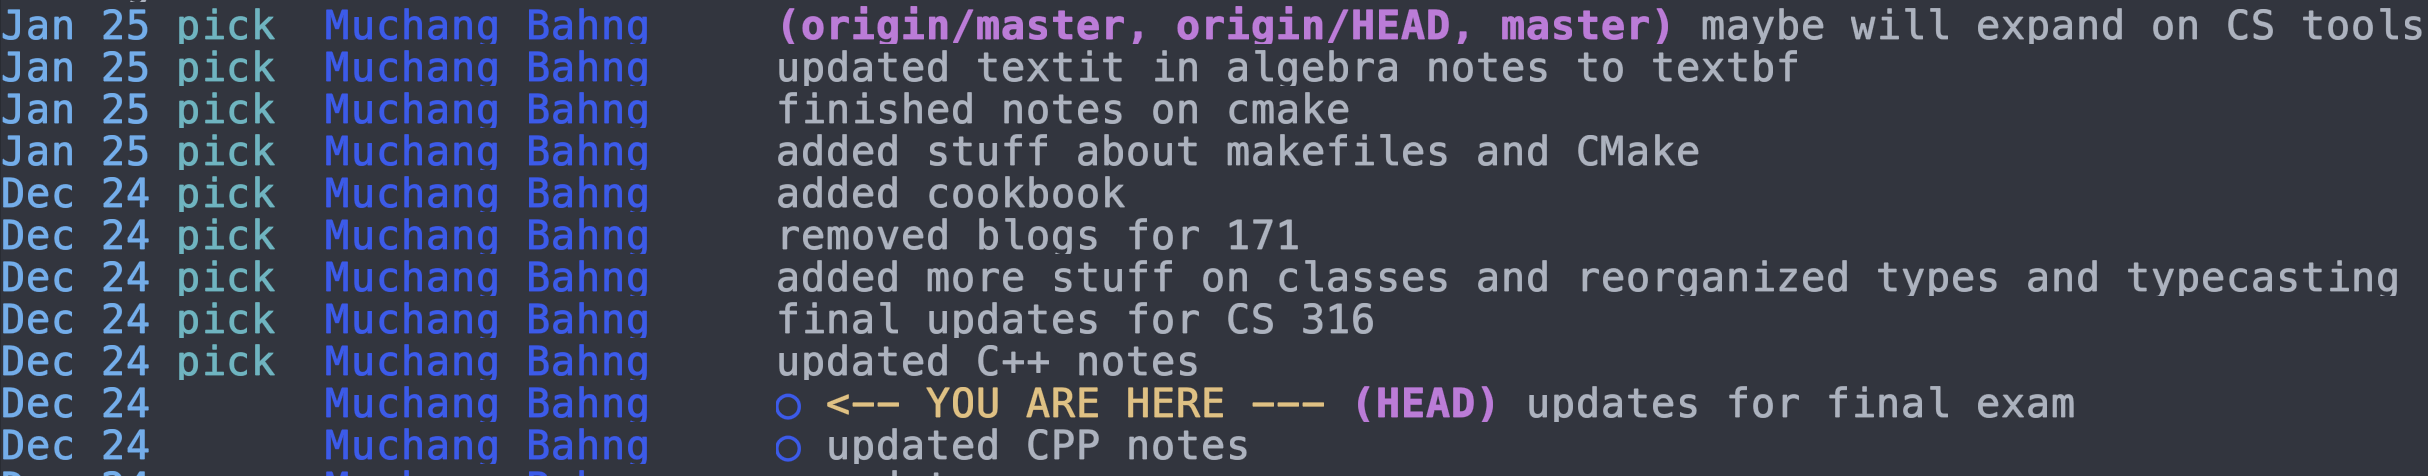
\includegraphics[scale=0.3]{img/rebase.png}
        \caption{Interactive rebase shown in LazyGit.} 
        \label{fig:rebase}
      \end{figure}

      There are a fixed set of supported operations allows in an interactive rebase.\footnote{Note that pick and reword will never cause conflicts. Squash and fixup will most likely not cause conflicts. Drop, break, edit, and swapping may cause conflicts.}
      \begin{enumerate}
        \item \textbf{Pick}. This just means that you are leaving the commit alone, i.e. picking it to be in the rebase. 
        \item \textbf{Reword}. Just edits the commit message. 
        \item \textbf{Squash}. Given commit $C_i \leftarrow C_{i+1}$, you can label $C_{i+1}$ with \texttt{squash} to merge it into $C_{i}$, turning 2 nodes into one. This almost never causes conflicts. The new commit message is just those of $C_{i}, C_{i+1}$ concatenated. 
        \item \textbf{Fixup}. Like squash, but discard the commit's message.  
        \item \textbf{Drop}. This deletes a commit and removes it entirely.  
        \item \textbf{Break}. Stop at this commit to edit it. I think you can change which edits you have committed, choose which edits to keep, and choose which edits to remove (back into your unstaged changes). 
        \item \textbf{Edit}. Stop at this commit to amend it. 
        \item You can also swap commits by editing the text file so that the commits are in a different order. 
          \begin{lstlisting}
            # Original order in rebase editor:
            pick abc123 First commit
            pick def456 Second commit

            # After swapping lines in editor:
            pick def456 Second commit
            pick abc123 First commit 
          \end{lstlisting}
      \end{enumerate} 
      After you edit the rebase text file and continue the rebase, git will do the following sequentially: 
      \begin{enumerate}
        \item \texttt{HEAD}, which pointed at $C_n$, will point towards $C_s$. 

        \item While \texttt{HEAD} is pointing at $C_i \neq C_n$ (i.e. not at the end), we do the following. 
          \begin{enumerate}
            \item It will attempt to perform all the operations you have specified for the next commit $C_{i+1}$. 
            \item If the operations are finished, we increment \texttt{HEAD} to point to $C_{i+1}$ and continue. 
            \item If there is a conflict, it will pause, state that there are conflicts between $\texttt{HEAD} = C_i$ and $C_{i+1}$, and ask you to resolve them. Once resolved it will continue. 
          \end{enumerate} 

        \item Then we are done with the rebase since we have went through all commits, modified them, and resolved all conflicts. 
      \end{enumerate}
      Interactive rebasing is an extremely powerful way to modify your commit history, and it's probably the operation where you'll spend the most time on git. 
    \end{definition} 

    Again, note that if you have changed anything in commit $C_i$, then the hash of $C_i$ every $C_j$ after will get changed. This causes git to interpret these changed commits as completely new ones, even if we only picked a given commit without any modifications. For single-branch rebases, this is fine, but this causes some nasty problems when rebasing over multiple branches, as we will talk about later. 

    \begin{definition}[Patching]
      An easier way to modify your edits in old commits is through \textbf{patching}.\footnote{Though patching really just does an interactive rebase in the backend.} Within a commit, a \textbf{patch} is simply a diff file that you can add and remove to. It's like having a mini-staging area in a commit. When you have selected the different files/lines you have added to your patch, you can either choose to: 
      \begin{enumerate}
        \item Remove them from the commit. 
        \item Add them to another commit. 
        \item Move them from the original commit to a new commit. 
      \end{enumerate}
    \end{definition}

    \begin{theorem}[Splitting Commits Into Two Different Commits]
      If you want to split commits, 
      \begin{enumerate}
        \item create a dummy commit 
        \item go to the commit you want to split, get its patches, and add them to the dummy commit. 
        \item Do an interactive rebase to swap the dummy commits down until you have it at the desired location. 
      \end{enumerate}
    \end{theorem} 

  \subsection{Branches} 

      Okay, so we now have much better control over our git history, but we've only been treating our history as a linked list. In order to introduce the tree structure, we need to introduce the \textit{branch}. This is especially important if we have a particular previous commit $C_{k < n}$ where we would like to make some different changes to, giving us \textbf{diverging histories} with next nodes $C_k \leftarrow C_{k+1}$ and $C_k \leftarrow C_{k^\prime + 1}$. 
      
      \begin{definition}[Branch]
        A \textbf{branch} is a path from the root commit to any leaf node. It represents a unique history from genesis to \texttt{HEAD}. To list all branches, use 
        \begin{lstlisting}
          >> git branch 
            feature/threading
          * main
            test/tensor
        \end{lstlisting} 
        The asterisk represents which branch you are currently on. The first branch you start off with is a special branch called \textbf{main}, or \textbf{master} branch. 
      \end{definition} 

      Therefore, really our linked-list history is a git tree with a single branch. 

      \begin{definition}[Creating/Switching Branches]
        From any (main or non-main) branch you can create new branches by choosing the commit to split from. 
        \begin{enumerate}
          \item Create a new branch from HEAD of current branch. 
            \begin{lstlisting}
              git branch <new-branch-name> 
            \end{lstlisting}

          \item Create a new branch from certain commit of current branch. 
            \begin{lstlisting}
              git branch <new-branch-name> <commit-hash>
            \end{lstlisting} 

          \item To switch to another branch 
            \begin{lstlisting}
              git checkout <branch> 
            \end{lstlisting}
        \end{enumerate}
      \end{definition} 

    \subsubsection{Working Between Branches} 

      If you are simultaneously working on multiple branches, you may have to checkout/switch between branches frequently. Often, you may have uncommitted changes before you checkout, and git does not allow you to do this. Therefore, we can \textit{stash} them. 

      \begin{definition}[Stash]
        \textbf{Stashing} changes mean that you can take uncommitted changes and store them in a temporary node but not have it point to any existing commit in a branch. This allows you to save your changes without having to commit incomplete work to a branch, and you can pop them back whenever you need. 
      \end{definition} 

      Sometimes, you may want to just copy a commit from one branch to another. You can do this using an interactive rebase, but this may be overkill since it is mainly used to work with a sequence of commits. 

      \begin{definition}[Cherry-Picking and Pasting]
        You can do copy a commit by \textbf{cherry picking} it and \textbf{pasting} it somewhere else. 
      \end{definition} 

    \subsubsection{Integrating Branches} 

      The reason you want to have different branches is so that you have independent workflows that may hopefully be integrated into the master branch. So how does one actually perform this integration? There are two general ways to do this: a 3-way merge or a rebase. For both methods, we will use this example. 
      \begin{lstlisting}
        main     : A1 --- A2 --- A3
                                  \
        feature1 :                 B1 --- B2 --- B3
                                  \
        feature2 :                 C1 --- C2 --- C3
      \end{lstlisting}

      \begin{definition}[Fast-Forward Merge]
        If you want to merge \texttt{main} and \texttt{feature1}, notice that \texttt{feature1} is really just ahead of \texttt{main} by some number of commits. The easiest way to merge is to add the additional commits in \texttt{feature1} to \texttt{main}. This is called a \textbf{fast-forward merge}, which we can call using 
        \begin{lstlisting}
          git checkout main 
          git merge --ff-only feature1
        \end{lstlisting} 
        Doing so will result in 
        \begin{lstlisting}
          main     : A1 --- A2 --- A3 --- B1 --- B2 --- B3
                                    \
          feature1 :                  --- B1 --- B2 --- B3
                                    \
          feature2 :                  --- C1 --- C2 --- C3
        \end{lstlisting}
        and we can delete \texttt{feature1} since it's not needed. 
      \end{definition}

      In fact, if a fast-forward merge is possible, then calling \texttt{git merge feature1} will automatically do a fast-forward. We can explicitly set it to only attempt or never attempt fast-forward by adding the \texttt{--ff-only} or \texttt{--no-ff} flags. 

      \begin{definition}[3-Way Merge]
        If you want to merge two divergent branches, e.g. \texttt{feature1} and \texttt{feature2}, then a fast-forward is not possible. Rather, you want to choose to merge \texttt{feature2} \textit{into} \texttt{feature1}. Git will rather do a \textbf{three-way merge} between the divergent node \texttt{A3} and the heads of the respective branches \texttt{B3} and \texttt{C3}. After you resolve conflicts, the tree should look something like 
        \begin{lstlisting}
          main     : A1 --- A2 --- A3
                                    \
          feature1 :                  --- B1 --- B2 --- B3 --- M1
                                    \                          /
          feature2 :                  --- C1 --- C2 --- C3 ---
        \end{lstlisting}
        Note that we could choose to merge \texttt{feature1} into \texttt{main} subsequently, resulting in both feature branches merged. 
        \begin{lstlisting}
          main     : A1 --- A2 --- A3 ------------------------------- M2
                                    \                                 /
          feature1 :                  --- B1 --- B2 --- B3 --- M1 ---
                                    \                          /
          feature2 :                  --- C1 --- C2 --- C3 ---
        \end{lstlisting}
      \end{definition}

      Note that a three-way merge may result in a pretty ugly tree, especially if we are working with dozens of branches. What we would like to do is a three-way merge in a fashion that \textit{looks like} a fast-forward merge. That is, we want the main branch to have a linear structure rather than a series of diverging and converging nodes. In fact, we already have the tools to do this. Let's revisit the interactive rebase again. We have seen that we can do an interactive rebase from a start commit by doing 
      \begin{lstlisting}
        git rebase -i <start-commit-hash>
      \end{lstlisting} 
      What we would like to do is to rebase from a commit in a different branch. 

      \begin{definition}[Rebase]
        If we want to linearly merge \texttt{feature2} into \texttt{feature1}, this is called ``\textbf{rebasing} \texttt{feature2} \textit{onto} \texttt{feature1}.'' We run 
        \begin{lstlisting}
          git checkout feature2 
          git rebase feature1
        \end{lstlisting} 
        which means ``take my current branch's unique commits and replay them on top of whatever branch I am rebasing on (in here, \texttt{feature1}).'' This will result in 
        \begin{lstlisting}
          main     : A1 --- A2 --- A3
                                    \
          feature1 :                 B1 --- B2 --- B3
                                                    \
          feature2 :                                 C1' --- C2' --- C3' 
        \end{lstlisting} 
        where the \texttt{C'} are the same commits but with different hashes since they start from a different parent. 
      \end{definition} 

      \begin{example}[Updating Feature Branch with Changes from Main]
        A common workflow you would do in a large project with multiple developers is as follows. Consider that you are working on \texttt{feature1} and another developer is working on \texttt{feature2}. 
        \begin{lstlisting}
          main     : A1 --- A2 --- A3
                                    \
          feature1 :                  --- B1 --- B2 --- B3
                                    \
          feature2 :                  --- C1 --- C2 
        \end{lstlisting}
        Your friend pushes their changes to \texttt{main}, which leads to this structure. 
        \begin{lstlisting}
          main     : A1 --- A2 --- A3 --- C1 --- C2
                                    \
          feature1 :                  --- B1 --- B2 --- B3
                                    \
          feature2 :                  --- C1 --- C2 
        \end{lstlisting}
        Your branch has diverged from main, so you will need to rebase your own branch onto main. You checkout to \texttt{feature1} and run \texttt{git rebase main}. After settling conflicts, your branch will look like the following, updated with the most recent commits from \texttt{main}. 
        \begin{lstlisting}
          main     : A1 --- A2 --- A3 --- C1 --- C2
                                                  \
          feature1 :                                --- B1' --- B2' --- B3'
                                    \
          feature2 :                  --- C1 --- C2 
        \end{lstlisting}
      \end{example}

      \begin{example}[Converting a Merge Into Rebase]
        Say that you already merged \texttt{feature1} and \texttt{main}. 
        \begin{lstlisting}
          main     : A1 --- A2 --- A3 ------------------------ M1
                                    \                          /
          feature1 :                  --- B1 --- B2 --- B3 ---  
        \end{lstlisting}
        You realized that you actually wanted to do a fast-forward so that it looks linear! How do you do this? 
        \begin{enumerate}
          \item You first undo the merge. 
            \begin{lstlisting}
              git checkout main 
              git reset --hard A3
            \end{lstlisting} 

          \item Then do the rebase of \texttt{feature1} onto \texttt{main}. 
            \begin{lstlisting}
              git checkout feature1 
              git rebase main 
            \end{lstlisting} 

          \item Then fast-forward to main to include \texttt{feature1}'s commits. 
            \begin{lstlisting}
              git checkout main 
              git merge --ff-only feature1
            \end{lstlisting}
        \end{enumerate}
        We will have this in the end. 
        \begin{lstlisting}
          main     : A1 --- A2 --- A3 --- B1' --- B2' --- B3' 
          feature1 : A1 --- A2 --- A3 --- B1' --- B2' --- B3'
        \end{lstlisting}
      \end{example} 

  \subsection{Remote Trees}

    So far, we've talked about how you can use git to keep track of your edit history locally, but another benefit is to store these changes in the cloud. This is done through a third-party provider, and they are completely separate entities from git. The three most dominant ones are  
    \begin{enumerate}
      \item \textit{Github}. Owned by Microsoft and is the default for most open-source projects, with 100 million users. 
      \item \textit{Gitlab}. Owned by Gitlab and is slowly gaining popularity due to better control of repositories and after Microsoft acquired github. 
      \item \textit{Bitbucket}. Owned by Atlassian and used for private repositories in enterprise settings. 
    \end{enumerate}
    Again, all three platforms still use \textit{git}, but the cloud storage is managed separately. All of these platforms provide a remote server that stores all of these git histories of millions of repositories around the world. The motivation behind the need of a remote workspace is that it is a common ground in which many developers can communicate and track the progress of their entire repository. 

    \begin{definition}[Remote Repository]
      The first step to setting up a cloud-based git tree is to place it on some server (IP address) in some directory with the proper permissions. This remote location containing the git tree and the corresponding code is called the \textbf{remote repository}, and it is encoded in either a URL or a SSH host link of the form 
      \begin{lstlisting}
        https://github.com/user/repo.git
      \end{lstlisting} 
      For now, we will consider a local repository having at most 1 remote repository that it can communicate to.\footnote{When we get to forking, we will talk about multiple remote repositories.} Conventionally, the primary\footnote{Again, for now it's really the only remote.} remote repository goes under the alias \textbf{origin}. 
    \end{definition}  

    None of the commands that we have introduced so far does anything to the remote repository. The first command we should know is how to set up one from scratch. 

    \begin{definition}[Add Remote]
      Given that git is initialized, we can initialize a corresponding remote repository by running 
      \begin{lstlisting}
        git remote add <remote-name> <remote-url>
      \end{lstlisting}
      Again, conventionally the \texttt{<remote-name>} is put as \texttt{origin}. 
    \end{definition} 

    Great, we have set a remote repository up, but there is an extra step to do. Most synchronizations happens at a branch level rather than the whole tree itself, so what we would need to do for each local branch is create a corresponding remote branch and then \textit{connect} those two so that git knows which branches to sync together. The local branch is called the \textbf{downstream} branch and its corresponding remote branch is called \textbf{upstream}. 

    In order to understand how the process of setting upstream branches is done, we introduce another variable in our local repository. In our local git tree, we have stated that for each branch \texttt{B}, there is a \texttt{HEAD} pointer living at the most recent commit, denoted as \texttt{B/HEAD} or just \texttt{B}. 

    \begin{definition}[Remote References] 
      There is actually a second pointer called the \textbf{remote reference (ref)} in the local branch called \texttt{origin/B} (more generally \texttt{<remote>/<branch>}), which is a symbolic link that points to the head of the remote branch. They are git's way of keeping track of the state of branches in your remote repositories. 
    \end{definition} 

    For some local branch, the existence of a remote ref tells you where the corresponding upstream branch is located (i.e. at \texttt{<remote>/<branch>}). If you do not see the remote ref, this means that you have not yet connected your local branch to its remote upstream, which can happen if the remote counterpart doesn't exist (i.e. you created a completely new branch) or you have never connected it. You can find all local branches and the remote references by calling 
    \begin{lstlisting}
      git branch -vv
      # Shows all branches with their tracking info
      # Example output:
      # * main    abc123 [origin/main] Latest commit message
      #   feature def456 [origin/feature: ahead 2] Some work
    \end{lstlisting} 

    \begin{definition}[Push with Set Upstream] 
      We consider two cases, where we do not see the remote refs at all. 
      \begin{enumerate}
        \item Say that you have a local branch \texttt{main} with some committed changes, and the remote branch does not exist at all. Your tree will look something like this 
          \begin{lstlisting}
            Remote: 
            Local : A <- B <- C <- (main) D
          \end{lstlisting}
        \item Say that you have a local branch \texttt{main} with some committed changes, and the remote branch does exist but the upstream is not set. 
          \begin{lstlisting}
            Remote: A <- (main) B
            Local : A <- B <- C <- (main) D
          \end{lstlisting}
      \end{enumerate}
      We can synchronize our local commits with the remote repo by \textbf{pushing} them. As we push, we also set the upstream with the \texttt{-u} or \texttt{--set-upstream} flag. 
      \begin{lstlisting}
        git push -u <remote> <branch> 
        
        # for example, if we want to push our current checked out branch to origin/main
        git push -u origin main
      \end{lstlisting}
      This will set your remote refs, and in both cases we will have 
      \begin{lstlisting}
        Remote: A <- B <- C <- (main) D
        Local : A <- B <- C <- (main, origin/main) D
      \end{lstlisting}
    \end{definition}

    \begin{definition}[Push] 
      If your remote ref is already set and you have some further commits, 
      \begin{lstlisting}
        Remote: A <- B <- C <- (main) D
        Local : A <- B <- C <- (origin/main) D <- E <- (main) F
      \end{lstlisting}
      then you can just push your changes with \texttt{git push}, which will push the commits up to HEAD and update the remote ref to HEAD. 
      \begin{lstlisting}
        Remote: A <- B <- C <- D <- E <- (main) F
        Local : A <- B <- C <- D <- E <- (main, origin/main) F
      \end{lstlisting}
    \end{definition} 

    In all of these scenarios, we have only seen cases when \texttt{origin/main} and \texttt{main} point to the same commit. However, remember that the remote ref is a \textit{local} pointer to the remote repo's head, and so it is only updated every time your local repo interacts with the remote repo. Therefore, they can be different. 

    \begin{example}[Remote Ref is Different From True Remote Head]
      Say that you are \texttt{Local1} and a friend is \texttt{Local2}. We first start off with this. 
      \begin{lstlisting}
        True Remote: A <- B <- C <- (main) D
        Remote1    : A <- B <- C <- (main) D 
        Local1     : A <- B <- C <- (main, origin/main) D 
        Remote2    : A <- B <- C <- (main) D
        Local2     : A <- B <- C <- (main, origin/main) D
      \end{lstlisting}
      Your friend makes commits \texttt{E} and \texttt{F} and pushes them while you are working on commit \texttt{G}.  
      \begin{lstlisting}
        True Remote: A <- B <- C <- D <- E <- (main) F
        Remote1    : A <- B <- C <- (main) D 
        Local1     : A <- B <- C <- (origin/main) D <- (main) G
        Remote2    : A <- B <- C <- D <- E <- (main, origin/main) F 
        Local2     : A <- B <- C <- D <- E <- (main, origin/main) F 
      \end{lstlisting} 
      In this case, your friend's push will update the head of the remote main branch to \texttt{F} and update their remote ref to \texttt{F} as well. But you have worked only locally and have no interacted with the remote repo for a while, so your remote ref is still \texttt{D}. When you therefore try to push your changes, git will complain to you that your future ref and the remote head does not match. Since this creates divergent histories which splits from \texttt{D}, it will not let you push. 
    \end{example}

    The scenario above is clearly a problem, and it stems from the fact that we have a remote ref. Why need remote refs at all if they seem redundant and at the same time they might introduce this problem? The answer is convenience. Imagine that there were no remote refs. This means that every time someone pushed to the remote main I would need to be notified that there were changes to main. However, I may not have access to the remote repo while I am working on my code, so I may still have the same problem when I am able to connect. The extra remote ref pointer allows for quick checking to see if my local branch matches its upstream. It turns out that if the upstream changed, git does indeed warn you about it as soon as possible. 

    \begin{definition}[Fetch] 
      Say that for a branch, it looks like this, and your local remote is not updated with the true remote's latest commits. 
      \begin{lstlisting}
        True Remote: A <- B <- C <- D <- E <- (main) F
        Remote1    : A <- B <- C <- (main) D 
        Local1     : A <- B <- C <- (origin/main, main) D
      \end{lstlisting}
      To update your remote ref to match the current upstream head, we can \textbf{fetch} it to get the following. 
      \begin{lstlisting}
        True Remote: A <- B <- C <- D <- E <- (main) F
        Remote1    : A <- B <- C <- D <- E <- (main) F
        Local1     : A <- B <- C <- (main) D <- E <- (origin/main) F
      \end{lstlisting}
      It comes in three commands. 
      \begin{lstlisting}
        git fetch <remote-url> <branch> # fetches from specific remote branch 
        git fetch <remote-url>          # fetches from all branches in a remote repo  
        git fetch                       # fetches from all branches of all remote repos
      \end{lstlisting}
    \end{definition}

    \begin{definition}[Fast-Forward]
      In the case above, note that even though the commits are synchronized to your local remote, the changes aren't actually reflected in your current code since HEAD has not moved. If you want head to also move to the most recent remote ref, then you can do a \textbf{fast-forward merge}. 
      \begin{lstlisting}
        True Remote: A <- B <- C <- D <- E <- (main) F
        Remote1    : A <- B <- C <- D <- E <- (main) F
        Local1     : A <- B <- C <- D <- E <- (origin/main, main) F
      \end{lstlisting}
      You can do this in git by checking out to the local branch you are on. After fetching, you should have the remote ref that you want to update your HEAD to, which you put in as an argument. 
      \begin{lstlisting}
        git merge --ff-only <remote-url/branch> 
        # e.g. 
        git merge -ff-only origin/main 
      \end{lstlisting}
    \end{definition}

    \begin{definition}[Pull]
      The combination of doing a fetch to get the latest commits and update the remote ref, and then doing a (fast-forward) merge to update your HEAD pointer to the remote ref, is so common that we refer to doing these two things sequentially as a \textbf{pull}. Therefore, the two commands are the same. 

      \noindent\begin{minipage}{.5\textwidth}
        \begin{lstlisting}[]{Code}
          git pull <remote-url> <branch> 

          git fetch <remote-url> <branch>  
          git merge <remote-url/branch>
        \end{lstlisting}
        \end{minipage}
        \hfill
        \begin{minipage}{.49\textwidth}
        \begin{lstlisting}[]{Output}
          git pull origin main 

          git fetch origin main 
          git merge origin/main
        \end{lstlisting}
      \end{minipage}
    \end{definition}

    \begin{definition}[Clone]
      Finally, you can take an existing remote repository and \textbf{clone} it, which creates a complete copy of a remote repository. It does the following. 
      \begin{enumerate}
        \item Does a \texttt{git init} to set up git. 
        \item Does \texttt{git remote add origin <remote-url>} to connect to the remote repo and set the \texttt{origin} alias to it. 
        \item Does \texttt{git fetch origin} to fetch all branches of the remote repo, setting up the local remote branches and their corresponding remote refs. 
        \item Does \texttt{git checkout -b main origin/main} which creates the local branch \textbf{main}, checks out to it, and sets \texttt{origin/main} as its upstream. 
      \end{enumerate}
    \end{definition}

  \subsection{Reflog} 

    \begin{definition}[Reflog]
      Git's \textbf{reflog} is a super-history that records every change to your branch tips. It's essentially an undo tree for all git actions (sort of like a meta undo tree). Therefore, if you ever screwed something up, git allows you to undo your actions by undoing the entries in the reflog. It contains the following types of actions. 
      \begin{enumerate}
        \item Branch Operations
          \begin{itemize}
            \item checkout: switching branches
            \item branch: creating/deleting branches
            \item merge: merging branches
            \item rebase: rebasing branches
            \item pull: pulling from remote
          \end{itemize}
        
        \item Commit Modifications
          \begin{itemize}
            \item commit: new commits
            \item reset: moving HEAD
            \item revert: reverting commits
            \item amend: amending commits
            \item cherry-pick: copying commits
          \end{itemize}

        \item Stash Operations
          \begin{itemize}
            \item stash: stashing changes
            \item stash apply: applying stash
            \item stash pop: popping stash
          \end{itemize}

        \item History Rewrites
          \begin{itemize}
            \item rebase -i: interactive rebase
            \item filter-branch: rewriting history
          \end{itemize}

        \item Reference Updates
          \begin{itemize}
            \item HEAD@{n}: moving HEAD pointer
            \item refs/heads/*: branch pointer updates
            \item refs/remotes/*: remote branch updates
            \item refs/stash: stash reference updates
          \end{itemize}

        \item Remote Operations
          \begin{itemize}
            \item clone: cloning repository
            \item fetch: fetching from remote
            \item push: pushing to remote
            \item remote add: adding remote
          \end{itemize}
      \end{enumerate}
      You can access it using the following command. 
      \begin{lstlisting}
        $ git reflog
        ab12345 HEAD@{0}: reset: moving to HEAD~1    # Most recent action
        bc23456 HEAD@{1}: commit: Add feature X 
        cd34567 HEAD@{2}: rebase: onto main          # Rebase happened here
        ef45678 HEAD@{3}: commit: Initial commit
      \end{lstlisting}
    \end{definition}

  \subsection{Pull Requests and Forking} 

\section{Continuous Integration (CI)} 

  \textbf{Continuous integration (CI)}, or \textbf{continuous development (CD)}, refers to any automated process that runs whenever you perform some action on a repository. These can include: 
  \begin{enumerate}
    \item Compiling your package upon pushing to a git branch. This saves the time of manually compiling it yourself. 
    \item Compiling and/or running unit tests on your package, over possibly different compiler/interpreter versions on different operating systems and different architectures, whenever someone opens a pull request. This is usually done by automatically creating docker images and running a script that sets up the environment for your system. 
    \item Automatically publishing a new package version to PyPI upon a push to the master branch of a repository. 
  \end{enumerate} 

  \textbf{Github actions} provide \textbf{workflow scripts} that you can include in your repository's \texttt{github/workflows/} directory that automates this. They are essentially yaml files that activate upon some command, whether that'd be a push to a branch, a pull request, or even the completion/failure of another workflow. This gives great convenience in deploying code. 

\section{Unittesting}

\section{Package Management} 

    Package management is quite a broad term, but for applications I will talk about them in the context of using Python, JavaScript, and C++. 

  \subsection{Pip} 

    Let's start off with a bit of history of Python, which was launched in 1991. 9 years later, the \textit{Python Distribution Utilities (distutils)} module was first added to the Python 1.6.1 standard library (and a month later, in Python 2.0), with the goal of simplifying the process of installing third-party Python packages. However, \texttt{distutils} only provided the tools for packaging Python code, but Python still lacked a centralized catalogue for packages on the internet. As a result, PEP 241 proposed to standardize metadata for packages, and in 2003, the \textit{Python Package Index (PyPI)} was finally launched. As of May 2024, PyPI has over 500,000 packages.\footnote{Really anybody can upload their own, so many packages may contain malware.} Each package is in the form of source archives, called \textit{wheels}, that contain binary modules from a compiled language. 

    Naturally, there is a need for a package manager, and \textit{easy install} was one of the first ones. After its deprecation in 2004, a software engineer named Ian Bicking introduced \textit{pyinstall}, which was quickly renamed to \textit{pip}.\footnote{From several suggestions the creator received on his blog post, and it is a recursive acryonym for ``pip installs packages.''} He also created a virtual environment manager, called \textit{virtualenv}, or \textit{venv}. 

    \begin{example}[Managing VirtualEnvs]
      Here are some useful commands. 
      \begin{lstlisting}
        # Unix Commands
        > python -m venv myVenvName/        # create the venv
        > source myVenvName/bin/activate    # activate it  
        > pip freeze > requirements.txt     # export venv into txt file 
      \end{lstlisting}
    \end{example}

    \begin{example}[Manage Packages Inside Venvs]
      Here are some useful commands. 
      \begin{lstlisting}
        > pip list                          # list all packages  
        > pip install xxx                   # install package
        > pip install xxx==0.0.1            # install version of package 
        > pip uninstall xxx                 # uninstall package
      \end{lstlisting} 
      Some notes: 
      \begin{enumerate}
        \item Running \texttt{pip install packagename} will look at PyPI, find the relevant package, and install one of the precompiled wheels for the operating system/python version that you are using.  
        \item \texttt{pip uninstall} does not uninstall depedencies! There is no built-in support for this, which is a pity. The best way to do this is to pip freeze and look at the differences in the packages. 
      \end{enumerate}
    \end{example}
    
  \subsection{Conda}

    While pip was great for managing Python packages, the main problem was that they were all focused around python, neglecting non-Python library depedencies, such as HDF5, MKL, LLVM, etc. Therefore, they do not install files into Python's site-packages directory. Therefore, \textit{conda} was released to do more than what pip does: handle dependencies \textit{outside} of Python packages as well as Python packages themselves. To reiterate, pip is for Python packages only, while conda is language-agnostic and can install packages in R or C (though it is mainly focused on Python). 

    Now that we've gotten this clear, let's talk about \textit{Anaconda}. In 2012, the company Anaconda Inc. was founded and created the \textit{Anaconda} and \textit{Miniconda} distributions mainly focused on data science and AI project for Python and R. You can think of them having the two main components. 
    \begin{enumerate}
      \item Access to the \textit{Anaconda Public Repository}, which consists of about 8000 packages (similar to PyPI). 
      \item A package manager called \textit{conda}, used to install/uninstall/modify these packages in virtual environments. 
    \end{enumerate}
    So the APR/conda is analogous to PyPI/pip. Furthermore, when you install Anaconda, a collection of about 300 essential packages (e.g. numpy, scipy, pandas) come pre-installed. This allows beginners to set up environments quickly with these essential packages but can come with a lot of bloat. There is also some GUI tools that are installed but are not really essential. Miniconda does not pre-install anything, so every new environment is completely empty. 

    \begin{example}[Manage Conda Envs]
      \begin{lstlisting}
        > conda env list                            # list all envionments
        > conda env create -n envname               # create new conda env with name 
        > conda env create -n envname python=3.9    # create new conda env with specific python version
        > conda env remove -n envname               # remove conda env
        > conda env export > environment.yaml       # export conda environment to yaml 
        > conda create -f environment.yaml          # make conda env from yaml file 
      \end{lstlisting}
    \end{example}

    Unlike PyPI, the Anaconda repository is divided into \textit{channels}, which are specific links that contain some subfamily of packages. The two most popular ones to know are: 
    \begin{enumerate}
      \item \texttt{default}: The default channel that is always there for the essentials. 
      \item \texttt{conda-forge}: A free open-source channel containing about 30,000 packages (as of May 2025). Anybody can contribute to this channel. 
    \end{enumerate} 

    \begin{example}[Manage Conda Channels]
      There are global commands that affect all conda environments. This can also be changed in your \texttt{.condarc} file, where the channels are listed from highest priority (top) to lowest (bottom). 
      \begin{lstlisting}
        > conda config --add channels some-channel        # add a channel permanently to ALL envs 
        > conda config --remove channels some-channel     # remove channel only to current env 
      \end{lstlisting}

      The following commands are for env-specific settings. 
      \begin{lstlisting}
        > conda config --show channels                          # show channels for current env
        > conda config --env --add channels some-channel        # add channel only to current env 
        > conda config --env --remove channels some-channel     # remove channel only to current env 
      \end{lstlisting}
    \end{example} 
    
    \begin{example}[Manage Packages Inside Conda Envs]
      Now that we know about channels, we can talk about installing packages. 
      \begin{lstlisting}
        > conda install packagename                         # install package 
        > conda install packagename=0.0.1                   # install specific version of package
        > conda install -c channel packagename              # install package from channel
        > conda uninstall packagename                       # uninstall package with dependencies
        > conda uninstall packagename --force               # uninstall package only without dependencies
        > conda uninstall --all --keep-env                  # uninstall all packages in env
      \end{lstlisting}
      Note that: 
      \begin{enumerate}
        \item Conda uses one \texttt{=} sign rather than pip, which uses \texttt{==}. 
        \item Conda actually supports both \texttt{uninstall} and \texttt{remove} keywords, unlike pip which only supports \texttt{uninstall}. 
        \item \texttt{conda remove} will remove all dependencies that are not used by other packages, which is nice. 
      \end{enumerate}
    \end{example}

  \subsection{Using Pip with Conda} 

    Now we go to the question that I have asked myself countless times, but have never took the time to study it until now. What is the difference between \texttt{pip install} and \texttt{conda install}? How should I use them together? To determine this, let's compare their behavior.  

    \begin{example}[Fresh Environment]
      Note that there is always \texttt{pip} installed in a venv while nothing is installed in a conda env. Since the \texttt{conda list} is quite verbose, I will exclude the \texttt{Build} and \texttt{Channel} colummns from now on. 

      \noindent\begin{minipage}{.25\textwidth}
        \begin{lstlisting}[]{Code}
          > pip list
          Package Version
          ------- -------
          pip     25.0.1 
        \end{lstlisting}
        \end{minipage}
        \hfill
        \begin{minipage}{.74\textwidth}
        \begin{lstlisting}[]{Output}
          > conda list
          # packages in environment at /opt/miniconda3/envs/test:
          #
          # Name              Version         Build  Channel 
        \end{lstlisting}
      \end{minipage}
    \end{example}

    \begin{example}[Dependency Installation when Installing a Package]
      Now let's install a single package \texttt{numpy==2.1.0}. We can see that the pip list is very minimal and only lists Python-related dependencies, while conda list contains a bunch of non-Python dependencies (a total of 24). Note that pip was automatically installed as a dependency, so we can also run \texttt{pip list} in the conda env and get the same output as the one in the venv.  
      
      \noindent\begin{minipage}{.35\textwidth}
        \begin{lstlisting}[]{Code} 
          > pip install numpy==2.1.0
          > pip list
          Package Version
          ------- -------
          numpy   2.1.0
          pip     25.0.1
          .
          .
          .
          .
          .
          .
        \end{lstlisting}
        \end{minipage}
        \hfill
        \begin{minipage}{.64\textwidth}
        \begin{lstlisting}[]{Output}
          > conda install numpy=2.1.0
          > conda list
          # packages in environment at /opt/miniconda3/envs/test:
          #
          # Name                    Version      
          ...
          ncurses                   6.5         
          numpy                     2.1.0       
          openssl                   3.4.1       
          pip                       25.0.1      
          python                    3.13.2      
          ...
        \end{lstlisting}
      \end{minipage}
    \end{example}

    \begin{example}[Uninstalling Package]
      Say that we have \texttt{pandas} installed and take a look at the list.
      
      \noindent\begin{minipage}{.35\textwidth}
        \begin{lstlisting}[]{Code}
          > pip install pandas 
          > pip list 
          Package         Version
          --------------- -----------
          numpy           2.2.4
          pandas          2.2.3
          pip             25.0.1
          python-dateutil 2.9.0.post0
          pytz            2025.2
          six             1.17.0
          tzdata          2025.2
        \end{lstlisting}
        \end{minipage}
        \hfill
        \begin{minipage}{.64\textwidth}
        \begin{lstlisting}[]{Output}
          > conda install pandas 
          > conda list
          # packages in environment at /opt/miniconda3/envs/test:
          #
          # Name                    Version       
          ...
          numpy                     2.2.4         
          openssl                   3.4.1         
          pandas                    2.2.3         
          pip                       25.0.1        
          ...
        \end{lstlisting}
      \end{minipage}

      Now if we uninstall it, we can see that conda removes dependencies while pip doesn't. 

      \noindent\begin{minipage}{.35\textwidth}
        \begin{lstlisting}[]{Code}
          > pip uninstall pandas 
          > pip list
          Package         Version
          --------------- -----------
          numpy           2.2.4
          pip             25.0.1
          python-dateutil 2.9.0.post0
          pytz            2025.2
          six             1.17.0
          tzdata          2025.2
        \end{lstlisting}
        \end{minipage}
        \hfill
        \begin{minipage}{.64\textwidth}
        \begin{lstlisting}[]{Output}
          > conda uninstall pandas 
          > conda list
          # packages in environment at /opt/miniconda3/envs/test:
          #
          # Name                    Version        
          ca-certificates           2025.1.31      
          openssl                   3.4.1          
          .
          .
          .
        \end{lstlisting}
      \end{minipage}
    \end{example} 

    \begin{example}[Dependency Updating]
      Now say that we have \texttt{numpy==1.26.4} and \texttt{scipy==1.12.0} installed in our venv and conda env. 

      \noindent\begin{minipage}{.35\textwidth}
        \begin{lstlisting}[]{Code}
          Package Version
          ------- -------
          numpy   1.26.4
          pip     23.2.1
          scipy   1.12.0 
          .
          .
          .
          .
          .
          .
          .
          .
          .
        \end{lstlisting}
        \end{minipage}
        \hfill
        \begin{minipage}{.64\textwidth}
        \begin{lstlisting}[]{Output}
          # packages in environment at /opt/miniconda3/envs/test:
          #
          # Name                    Version   
          numpy                     1.26.4    
          openssl                   3.4.1     
          pip                       25.0.1    
          python                    3.12.9    
          python_abi                3.12      
          readline                  8.2       
          scipy                     1.12.0    
          setuptools                78.1.0    
          tk                        8.6.13    
          tzdata                    2025b     
          wheel                     0.45.1    
        \end{lstlisting}
      \end{minipage}

      We would like to upgrade numpy to 2.2.0, but this will break the dependency for scipy. Both package managers report this, and pip gives a more readable message. However, note that conda does not install \texttt{numpy=2.2.0}, while pip \textit{does} and reports that this can break things. So even though it checks for dependencies, it does \textit{not} automatically update them!

      \noindent\begin{minipage}{.35\textwidth}
        \begin{lstlisting}[]{Code}
          Package Version
          ------- -------
          numpy   2.2.0
          pip     23.2.1
          scipy   1.12.0 
          .
        \end{lstlisting}
        \end{minipage}
        \hfill
        \begin{minipage}{.64\textwidth}
        \begin{lstlisting}[]{Output}
          # packages in environment at /opt/miniconda3/envs/test:
          # Name                    Version   
          numpy                     1.26.4    
          pip                       25.0.1    
          python                    3.12.9    
          scipy                     1.12.0    
        \end{lstlisting}
      \end{minipage}
    \end{example}

    As we have seen there are two deal-breakers for pip, which is that it does not clean up dependencies upon installation and that it updates packages that may break dependencies. This is really because pip is a package manager, but it is \textit{not} a dependency manager. So personally, I only do pip install when it is absolutely necessary, i.e. I need a package that is only available on PyPI and not on any Anaconda channels. 

    \begin{theorem}[Best Practices for using Conda and Pip]
      Here are my personal best practices. 
      \begin{enumerate}
        \item Always use conda environments. 
          \begin{enumerate}
            \item Conda environments completely replace virtualenvs. There is nothing you can do in virtualenvs that you cannot do in conda envs. 
            \item Venvs only work with pip, while conda envs allow you to have access to conda, which can be used to download pip. 
            \item You cannot easily switch Python versions in an environment in venv, since you must have the binary installed on your computer. However for conda, it is as easy as \texttt{conda install python=3.x}. 
          \end{enumerate}
        \item Always use \texttt{conda install} if possible, and only use \texttt{pip install} if you need a package only on PyPI. This is for the following reasons. 
          \begin{enumerate}
            \item Due to dependency breaking as mentioned above (and elaborated below), pip can be a huge headache to work with.\footnote{Though most widely used packages are pretty good at making sure that there are no incompatibilities.} 
            \item Pip usually breaks more often when downloading more outdated packages. \footnote{For example, installing \texttt{pandas=1.1.4} works on conda but not with pip. }
          \end{enumerate}

          \item Whether you export your environment one way or another will depend on how flexible/rigid you want your working environment to be when you share. 
            \begin{enumerate}
              \item \texttt{conda env export} will keep track of every (including non-Python related) modules, and those imported with pip will be under the \texttt{pip} header. 
              \item \texttt{pip freeze} will only keep track of Python packages installed and can be cleaner. 
            \end{enumerate}
      \end{enumerate}
    \end{theorem}

    Others note that if you using conda environments, you should always just use \texttt{conda install}, and if you ever need to \texttt{pip install}, then just use \texttt{venv} and \texttt{pip install} everything. With venvs, if you ever see a dependency issue, don't try to resolve it: burn the whole environment down and recreate a new one from scratch. 

  \subsection{Mamba} 

    I've been using pip and conda for about 6 years before I found out about \textit{mamba} in a summer internship. The Mamba project began in 2019 as a thin wrapper around conda and has grown considerably by progressively rewriting conda with equivalent new efficient C++ code. It is estimated to be about 10 times faster in creating a large environment from scratch compared to conda. There are essentially no strict disadvantages to using mamba, but due to its newness it is still relatively unpopular. So besides the fact that mamba support is lower, it might be good to try it as a replacement. It also seems that recently (as of May 2025), conda caught up to the speed of mamba, so it also may not be worth switching. I'll have to run some tests for this. 

    The bigger consideration is that for many users (such as companies with 200+ employees), Anaconda Inc. starting from 2020 required paid licensing for commercial use, including any use of the \texttt{defaults} channels (though \texttt{conda-forge} channel remains free). 

\end{document}
